\chapterimage{slike/Laguerre.jpg} % Chapter heading image

\chapter{Koherentni snopi svetlobe}
V tem poglavju bomo zapisali obosni približek valovne enačbe in spoznali 
njeno osnovno rešitev: Gaussov snop. Obravnavali bomo snope osnovnega in višjega reda ter
se naučili računati prehode Gaussovih snopov skozi optične elemente. 

\section{Omejen snop svetlobe}
Pri obravnavi elektromagnetnega valovanja pogosto uporabljamo
približek ravnih valov\index{Ravni val}. Ti so v smeri pravokotno na smer širjenja
neomejeni in so zato lahko le idealizacija. Čim raven val usmerimo skozi odprtino
v zaslonu, nastane omejen snop svetlobe\index{Omejen snop}. V snopu svetlobe valovna čela niso
ravna in meje snopa niso vzporedne, ampak se snop zaradi uklona širi\index{Uklon} 
(slika \ref{fig:Uklon-na-rezi}).
\begin{figure}[h]
\centering
\def\svgwidth{120truemm} 
\input{slike/03_uklon_na_rezi.pdf_tex}
\caption{Omejen snop nastane ob prehodu ravnega vala skozi končno odprtino.}
\label{fig:Uklon-na-rezi}
\end{figure}

V veliki oddaljenosti od zaslona polje izračunamo s
\index{Fraunhoferjev uklon}Fraunhoferjevo uklonsko teorijo (glej poglavje~\ref{FFuklon}). 
Vendar za oceno kota širjenja računa niti ne potrebujemo. Velja približno 
\begin{equation}
\vartheta\sim\frac{\lambda}{a},
\label{eq:kot_ocena}
\end{equation}
kjer je $a$ polmer odprtine v zaslonu.
Opis polja v bližini zaslona je zahtevnejši, saj je treba uporabiti 
Fresnelov približek\index{Fresnelov uklon} (enačba~\ref{eq:FresnelApprox}).
Območje bližnjega polja seže do $b$, ki ga lahko ocenimo s slike (\ref{fig:Uklon-na-rezi})
\begin{equation}
\frac{a}{b}\sim{\vartheta}\sim \frac{\lambda}{a} \qquad \mathrm{in~tako} \qquad b\sim\frac{a^2}{\lambda}.
\label{eq:z_ocena}
\end{equation}

Včasih taki približni oceni zadoščata. Bolj kvantitativen opis omejenih
snopov bi lahko dobili s Fraunhoferjevo in Fresnelovo uklonsko teorijo,
kar pa ni najudobnejša pot (glej nalogo~\ref{ffuklon}). Lotimo se problema raje z 
uporabo približka obosne valovne enačbe.

\begin{definition}
\label{ffuklon}
Pokaži, da je Fraunhoferjeva uklonska slika na odprtini, katere prepustnost se v radialni smeri
spreminja kot Gaussova funkcija $T(\xi, \eta)=e^{-(\xi^2+\eta^2)/w_0^2}$, podana z Gaussovo funkcijo
oblike $E(x,y,z) \propto e^{-(x^2+y^2)/w^2(z)}$ in določi odvisnost $w(z)$. Izračunaj še 
uklonsko sliko v bližnjem polju po Fresnelovi uklonski teoriji.
\end{definition}

\section{Obosna valovna enačba}
Obravnavo začnemo z valovno enačbo in monokromatskim valovanjem s krožno frekvenco $\omega$. Ustrezna
Helmholtzeva enačba je \index{Helmholtzeva enačba}(enačba~\ref{eq:Helmholtz})
\begin{equation}
\nabla^{2}E+k^{2}E=0,
\label{eq:valovna-enacba-hh}
\end{equation}
kjer je $k=n\omega/c_{0}$ valovno število in $n$ lomni količnik
sredstva, po katerem se valovanje širi. Zaradi enostavnosti obravnavamo
le eno polarizacijo, tako da $E$ pišemo kot skalar. Iščemo rešitev za
omejen snop, ki se širi približno vzdolž osi $z$. Uporabimo nastavek
\begin{equation}
E=E_{0}\psi(\mathbf{r},z)e^{ikz},
\label{eq:ravni-val-nastavek}
\end{equation}
kjer je $\mathbf{r}$ krajevni vektor v ravnini $xy$, prečni na smer širjenja svetlobe. 
Glavni del odvisnosti od koordinate $z$ smo zapisali v faktorju $e^{ikz}$, tako da lahko
privzamemo, da se $\psi$ v smeri $z$ le počasi spreminja. Vstavimo
gornji nastavek v Helmholtzevo enačbo (enačba~\ref{eq:valovna-enacba-hh})
in pri tem zanemarimo druge odvode $\psi$ po $z$, saj je zaradi počasnega spreminjanja
$\partial^{2}\psi/\partial z^{2}$ majhen v primerjavi s $k\partial\psi/\partial z$ in $k^{2}\psi$.
Dobimo obosno
ali paraksialno valovno enačbo\index{Obosna valovna enačba} za $\psi$
\index{Paraksialna enačba|see{Obosna valovna enačba}}
\boxeq{eq:obosna-valovna-enacba}{
\nabla_{\perp}^{2}\psi=-2ik{\frac{{\partial\psi}}{{\partial z}}}.
}
\begin{remark} 
Opazimo, da je obosna valovna enačba enaka Schr\"{o}dingerjevi enačbi
za prost delec v dveh dimenzijah, v kateri ima koordinata $z$ vlogo
časa. Omejenemu snopu v kvantni mehaniki ustreza lokaliziran delec
-- valovni paket. Ta se s časom širi, kar v optiki ustreza pojavu uklona.
\end{remark}
Zapišimo nastavek za ravni val \index{Ravni val} v obliki
\begin{equation}
\psi=e^{ik_{1}x+ik_{2}y}\, e^{-i\beta z}.
\label{eq:ravni-val-nastavek-obosni}
\end{equation}
Da bo gornji nastavek rešitev
obosne valovne enačbe~(enačba~\ref{eq:obosna-valovna-enacba}), mora veljati 
\begin{equation}
\beta=\frac{k_{1}^{2}+k_{2}^{2}}{2k}.
\end{equation}
Ko vstavimo nastavek za $\psi$ v izraz za polje $E$ 
(enačba~\ref{eq:ravni-val-nastavek}), dobimo ravni val, za katerega velja 
\begin{equation}
k_{3}=k-\beta=k-\frac{k_{1}^{2}+k_{2}^{2}}{2k}.
\label{eq:k3-razvoj}
\end{equation}
Pri tem $k_{3}$ označuje vzdolžno in $k_{1}$ ter $k_{2}$ prečni komponenti valovnega 
vektorja, $k$ pa je valovno število. 
Za ravni val, ki je rešitev Helmholtzeve enačbe (enačba~\ref{eq:valovna-enacba-hh})
in ne obosnega približka (enačba~\ref{eq:obosna-valovna-enacba}), velja 
\begin{equation}
k_{3}=\sqrt{k^{2}-(k_{1}^{2}+k_{2}^{2})}.\label{eq:k3-tocno}
\end{equation}
Vidimo, da sledi enačba~(\ref{eq:k3-razvoj}) iz enačbe~(\ref{eq:k3-tocno})
z razvojem za majhne vrednosti $k_1$ in $k_2$. To pove, da je približek obosne 
enačbe dober, kadar je razmerje prečne in vzdolžne komponente valovnega vektorja 
majhno. Takrat je majhen tudi kot širjenja snopa in člene, višje od kvadratnih,
lahko zanemarimo. To pa je tudi območje veljavnosti Fresnelove uklonske
teorije.\index{Fresnelov uklon}

\begin{remark}\index{Fouriereva optika}
Časovno odvisnost poljubnega začetnega
stanja v kvantni mehaniki navadno izračunamo tako, da v nekem začetnem
trenutku paket razvijemo po lastnih stanjih energije -- ravnih valovih.
Rešitev v poljubnem kasnejšem trenutku je potem dana v obliki Fourierevega
integrala. Ta pot je zelo uporabna tudi v optiki in je osnova sklopa
računskih metod, znanih pod imenom Fouriereva optika. V našem primeru
z njo brez težav pridemo nazaj do Fresnelove uklonske formule.
\end{remark}

\section{Osnovni Gaussov snop}
\index{Gaussov snop}
Naša naloga je poiskati rešitve obosne enačbe, ki popišejo omejene
snope. Iz kvantne mehanike vemo, da je najbolj lokaliziran in se najpočasneje
širi valovni paket Gaussove oblike. Zato poskusimo najti rešitev obosne
enačbe (enačba~\ref{eq:obosna-valovna-enacba}) z nastavkom
\begin{equation}
\psi(r,z)=e^{ikr^{2}/2q(z)}\, e^{-i\phi(z)},\label{eq:gaussov-snop-nastavek}
\end{equation}
kjer funkcija $q(z)$ opisuje širjenje snopa v prečni smeri,
$\phi(z)$ pa opisuje počasno spreminjanje faze snopa vzdolž osi $z$.
Vstavimo nastavek (enačba~\ref{eq:gaussov-snop-nastavek}) v obosno valovno enačbo 
(enačba~\ref{eq:obosna-valovna-enacba}). Zaenkrat se omejimo le na radialno 
simetrične rešitve in v cilindričnih koordinatah zapišemo
\begin{equation}
\nabla_{\perp}^{2}\psi=\frac{1}{r}\frac{\partial}{\partial r}\, r\,\frac{\partial\psi}{\partial r}=
\left( \frac{2ik}{q}-\frac{k^2r^2}{q^2}\right)\psi
\end{equation}
 in 
\begin{equation}
\frac{\partial\psi}{\partial z}=\left(-\frac{ikr^{2}}{2q^2}q(z)^{\prime}-i\phi^{\prime}\right)\psi.
\end{equation}
Tako iz obosnega približka (enačba~\ref{eq:obosna-valovna-enacba}) sledi
\begin{equation}
\frac{2ik}{q}-\frac{k^2r^2}{q^2}=ik\left(\frac{ikr^{2}}{q^2}q(z)^{\prime}+2i\phi^{\prime}\right).
\end{equation}
Gornja zveza mora veljati pri vsakem $r$, zato so koeficienti
pri $r^{2}$ na obeh straneh enačbe enaki in členi brez odvisnosti od $r$ prav tako. Sledi
\begin{equation}
q(z)^{\prime}=1\mbox{\hskip1cm in \hskip1cm}\phi^{\prime}=-\frac{i}{q}.
\end{equation}
Z integracijo dobimo najprej 
\begin{equation}
q=z-iz_{0},
\label{eq:alpha}
\end{equation}
kjer smo z $-i z_{0}$ označili integracijsko konstanto. 
Integriramo še enačbo za fazo 
\begin{equation}
\phi=\int_{0}^{z}\,-\frac{i dz}{z-iz_{0}}=-i\ln(1+i\frac{z}{z_{0}}).
\end{equation}
Sledi
\begin{eqnarray}
\psi & = & \exp\left(i\frac{kr^{2}}{2(z-iz_0)}\right)\,\exp\left(-\ln(1+i\frac{z}{z_{0}})\right)=
\nonumber \\
 & = & \frac{1}{1+i\frac{z}{z_{0}}}\,\exp\left(-\frac{kr^{2}z_{0}}{2(z_{0}^{2}+z^{2})}+
 \frac{ikr^{2}z}{2(z_{0}^{2}+z^{2})}\right).
 \label{eq:gaussov-snop-vmesni}
\end{eqnarray}
Najprej podrobneje poglejmo realni del eksponenta, ki opisuje širjenje snopa. Polmer snopa $w$, 
ki je funkcija koordinate $z$, opišemo z enačbo \index{Gaussov snop!polmer}
\begin{equation}
w^{2}=\frac{2z_{0}}{k}\left(1+\left(\frac{z}{z_{0}}\right)^{2}\right).
\end{equation}
V izhodišču pri $z=0$ je snop najožji in pravimo, da je tam grlo snopa\index{Gaussov snop!grlo}. 
Polmer snopa v grlu označimo z $w_0$ in zapišemo hiperbolično zvezo $w(z)$
\boxeq{eq:w}{
w^2 = w_{0}^{2}\left(1+\left(\frac{z}{z_{0}}\right)^{2}\right).
}
Pri tem velja 
\begin{equation}
w_0^2 = \frac{2z_0}{k}
\end{equation}
oziroma 
\boxeq{eq:z0}{
z_{0}=\frac{\pi w_{0}^{2}}{\lambda}.
}
Dolžina\index{Gaussov snop!dolžina grla} 
$z_{0}$ je razdalja, pri kateri preide snop v asimptotično enakomerno širjenje. 
Čeprav smo vpeljali grlo kot najožji del snopa (pri $z=0$), uporabljamo izraz grlo tudi 
za celotno območje, znotraj katerega se snop ne razširi znatno. Njegovo dolžino
določa ravno parameter $z_0$, tako da je dolžina celotnega grla $2z_0$. Območju grla 
pravimo območje bližnjega polja
\index{Območje bližnjega polja} ali Rayleighovo območje\index{Rayleighovo 
območje|see{Območje bližnjega polja}} in dolžini $z_0$ \index{Rayleighova dolžina}Rayleighova 
dolžina\footnote{Angleški fizik in nobelovec John William Strutt, 3. baron Rayleighški; lord
Rayleigh, 1842--1919.}.
Dolžina $z_{0}$ označuje tudi oddaljenost od grla, pri kateri začne veljati Fraunhoferjev uklonski približek. 
\begin{figure}[h]
\centering
\def\svgwidth{100truemm} 
\input{slike/03_Gauss.pdf_tex}
\caption{Gaussov snop s karakterističnimi parametri}
\label{fig:Gauss}
\end{figure}

Zapišimo še kot divergence snopa v velikih oddaljenostih. Polovični kot širjenja je
\begin{equation}
\vartheta=\lim_{z \to \infty} \frac{dw}{dz} = \frac{w_{0}}{z_{0}}=
\frac{\lambda}{\pi w_{0}}.\label{eq:divergenca-snopa}
\end{equation}
Celotna divergenca snopa\index{Gaussov snop!divergenca} pa
\boxeq{eq:divergenca-snopa2}{
\theta=2 \frac{w_{0}}{z_{0}}=\frac{2\lambda}{\pi w_{0}}.
}

Izraza za območje bližnjega polja (enačba~\ref{eq:z0}) in divergenco 
(enačba~\ref{eq:divergenca-snopa}) sta v skladu z ocenama, ki smo ju 
napravili v začetku poglavja (enačbi~\ref{eq:kot_ocena} in \ref{eq:z_ocena}). Faktor 
$1/\pi$ je značilen za Gaussov snop, ki ima od vseh možnih oblik 
najmanjšo divergenco. 

Za določanje kakovosti dejanskega laserskega snopa 
in njegovega odstopanja od idealnega Gaussovega snopa se pogosto vpelje faktor \index{Faktor $M^2$}$M^2$
\begin{equation}
\theta = M^2 \frac{2\lambda}{\pi w_{0}}.
\label{faktorM}
\end{equation}
Dobri laserji dosegajo vrednost $M^2 \sim 1$,
pri močnejših trdninskih ali polprevodniških laserjih pa je lahko $M^2 \sim 30$ ali več. 
V grobem velja, da $M^2$ narašča z močjo laserja in oblika snopa močnih laserjev navadno znatno
odstopa od oblike idealnega Gaussovega snopa.  

Vrnimo se k imaginarnemu delu eksponenta v enačbi~(\ref{eq:gaussov-snop-vmesni}).
Vpeljemo količino 
\boxeq{eq:R}{
R=z\left(1+\left(\frac{z_{0}}{z}\right)^{2}\right),
}
ki meri krivinski radij valovnih front\index{Gaussov snop!krivinski radij} 
pri oddaljenosti od grla $z$. To najlažje
uvidimo, če zapis imaginarnega dela primerjamo z zapisom za krogelni val, razvit 
po majhnih odmikih $r$ od osi
$z$
\begin{equation}
\frac{1}{R}e^{ikR}=\frac{1}{R}e^{ik\sqrt{z^{2}+r^{2}}}\approx \frac{1}{R}e^{ikz+ikr^{2}/2R}.
\label{eq:krogelni-val}
\end{equation}
Upoštevali smo, da je na osi $z=R$.

\begin{definition}
\label{naloga-ukrivljenost-snopa}
Pokaži, da je največja ukrivljenost valovnih front snopa (in s tem najmanjši $R$) ravno pri $z=\pm z_{0}$.
Izračunaj še ukrivljenost front v grlu in v veliki oddaljenosti od grla.
\end{definition}

Na sliki (\ref{fig:ravni-Gaussov-krogelni-val}) 
so prikazane valovne fronte ravnega vala, 
Gaussovega snopa (enačba~\ref{eq:gaussov-snop}) 
in krogelnega vala (enačba~\ref{eq:krogelni-val}). Vidimo, da je v grlu
Gaussov snop podoben ravnemu valu 
(ukrivljenost front je zelo majhna in $R \to \infty$). Za velike oddaljenosti
krivinski radij valovnih front postaja kar enak oddaljenosti $z$.
Snop je tako podoben delu krogelnega vala, le da je faza Gaussovega snopa 
zamaknjena za $\pi/2$ glede na krogelni val. 

\begin{figure}[h]
\centering
\def\svgwidth{70truemm} 
\input{slike/03_fronte.pdf_tex}
\caption{Ravni val, Gaussov snop ter
krogelni val. V grlu je Gaussov snop podoben ravnemu valu, 
pri velikih oddaljenostih od grla pa krogelnemu valu.}
\label{fig:ravni-Gaussov-krogelni-val}
\end{figure}

Ostane še faktor pred eksponentom v izrazu~(\ref{eq:gaussov-snop-vmesni}). Ta faktor meri
zmanjševanje amplitude električne poljske jakosti v snopu in s tem poskrbi za ohranitev energijskega
toka ob širjenju žarka, poleg tega pa še dodatno spremeni fazo. Zapišemo ga v obliki
\index{Gaussov snop!faza}
\begin{equation}
\frac{1}{1+i\frac{z}{z_{0}}}=\frac{1}{\sqrt{1+(\frac{z}{z_0})^{2}}}e^{-i\eta(z)}=\frac{w_{0}}{w}e^{-i\eta(z)},
\end{equation}
 pri čemer je
\boxeq{eq:eta}{
\eta(z)=\arctan\left(\frac{z}{z_{0}}\right).
}
Dodatna faza $\eta$, imenujemo jo tudi \index{Gouyeva faza}Gouyeva 
faza\footnote{Francoski fizik Louis Georges Gouy, 1854--1926.},
je posledica povečane fazne hitrosti valovanja,
kadar je valovanje omejeno v prečni smeri. Podoben pojav bomo srečali tudi pri valovanju, ki je 
omejeno v valovode (poglavje~\ref{chap:fibri}).

S tem lahko končno zapišemo izraz za električno poljsko jakost osnovnega \index{Gaussov snop}Gaussovega 
snopa\footnote{Nemški matematik, fizik in astronom Carl Friedrich Gauss, 1777--1855.}
\boxeq{eq:gaussov-snop}{
E(r,z,t)=E_{0}\,\frac{w_{0}}{w(z)}\,e^{ikz-i\omega t}\,e^{-r^{2}/w^{2}(z)}\,e^{ikr^{2}/2R(z)}
e^{-i\eta(z)}.
}

Intenziteta svetlobe\index{Gaussov snop!intenziteta} je sorazmerna z $E(r,z)E^*(r,z)$ in zanjo velja
\boxeq{eq:gaussov-snop-intenziteta}{
I(r,z)= I_{0}\,\frac{w_0^2}{w^2(z)}\,e^{-2r^{2}/w^{2}(z)}.
}

\begin{figure}[h]
\centering
\def\svgwidth{100truemm} 
\input{slike/03_Gauss_3D.pdf_tex}
\caption{Upodobitev intenzitete svetlobe v Gaussovem snopu za $z>0$ }
\label{fig:Gauss_3D}
\end{figure}

\begin{definition}
\label{naloga-širina-snopa}
Pokaži, da je celotna svetlobna moč v snopu enaka $P = \frac{1}{2}\pi w_0^2\, I_0$.
\end{definition}

Povejmo še nekaj o parametru $q(z)$, ki smo ga uporabili pri izračunu Gaussovega snopa v nastavku
(enačba~\ref{eq:gaussov-snop-nastavek}). Spomnimo 
se, da parameter $q$ narašča linearno z oddaljenostjo od grla
\begin{equation}
q(z) = z -iz_0.
\label{eq:q}
\end{equation}
Parameter $q$ imenujemo kompleksni krivinski radij\index{Kompleksni krivinski radij}, 
njegov inverz pa kompleksna ukrivljenost\index{Kompleksna ukrivljenost}
\boxeq{eq:q-inv}{
\frac{1}{q(z)}=\frac{1}{R}+i\frac{2}{kw^{2}}.
}
\begin{definition}
Uporabi enačbi (\ref{eq:z0} in \ref{eq:R}) in izpelji gornji izraz za kompleksno ukrivljenost.
\end{definition}
Izkazalo se bo, da je kompleksni krivinski radij zelo uporaben pri 
obravnavi preslikav Gaussovih snopov z lečami.

\section{Snopi višjega reda}

Osnovna rešitev obosne valovne enačbe (enačba~\ref{eq:obosna-valovna-enacba}) 
je Gaussov snop (enačba~\ref{eq:gaussov-snop}). Poleg te rešitve obstaja še veliko 
drugih rešitev, prav tako omejenih v prečni smeri. 
V kartezičnih koordinatah tako rešijo obosno valovno enačbo
\index{Hermite-Gaussovi snopi}Hermite-Gaussovi snopi\footnote{Francoski matematik Charles Hermite, 1822--1901.}
\begin{equation}
\psi_{n,m}(x,y)=\frac{w_{0}}{w}H_{n}\left(\frac{\sqrt{2}x}{w}\right)H_{m}\left(\frac{\sqrt{2}y}{w}\right)
\exp\left(\frac{ik(x^{2}+y^{2})}{2q}-i\eta_{n,m}\right),
\label{eq:Gauss-Hermitevi}
\end{equation}
kjer so $H_{n}$ Hermitovi polinomi stopnje $n$ (npr. $H_0(x)=1, H_1(x)=2x, H_2(x)=4x^2-2, H_3(x)=8x^3-12x$ ...). 
V to se lahko
prepričamo, če izraz vstavimo v obosno valovno enačbo\index{Obosna valovna enačba}
(enačba~\ref{eq:obosna-valovna-enacba}) in upoštevamo zvezo med Hermitovimi polinomi 
\begin{equation}
H_{n}^{\prime\prime}-2xH_{n}^{\prime}+2nH_{n}=0.
\end{equation}
Osnovni Gaussov snop je očitno poseben primer gornje rešitve za $n=m=0$.
Polmer snopa $w(z)$ in kompleksni krivinski radij $q(z)$ sta za
vse $n$ in $m$ enaka kot za osnovni snop in podana z enačbama (\ref{eq:w})
in (\ref{eq:q}). Razlika je v fazi, ki je odvisna tudi od $n$ in $m$\index{Gouyeva faza}
\begin{equation}
\eta_{n,m}\left(z\right)=(n+m+1)\arctan\left(\frac{z}{z_{0}}\right).
\end{equation}

Nekaj višjih redov Hermite-Gaussovih snopov je na sliki (\ref{fig:Gauss-Hermitevi-snopi}),
kjer rišemo $|\psi_{n,m}(x, y, 0)|$.
Indeksa $n$ in $m$ določata število vozlov v prečnih smereh $x$ in $y$,
širina snopa pa narašča z $n$ in $m$. 

\begin{figure}[h]
\centering
\def\svgwidth{110truemm} 
\input{slike/03_Hermite_Gauss.pdf_tex}
\caption{Prečni profil absolutne vrednosti električne poljske jakosti
Hermite-Gaussovih snopov v grlu za različne vrednosti $(n,m)$}
\label{fig:Gauss-Hermitevi-snopi}
\end{figure}

\begin{definition}
\label{naloga:HG}
Pokaži, da za Hermite-Gaussove snope višjih redov efektivni polmer snopa 
narašča sorazmerno s korenom iz števila prečnih vozlov $ w_{eff}\propto w\sqrt{n+m}$.\\
Namig: pri zapisu prečne odvisnosti polja upoštevaj le vodilni člen
 Hermitovih polinomov in določi razdaljo od središča snopa, pri kateri je 
 amplituda polja $\psi$ največja.
\end{definition}

\begin{remark}
 Hermite-Gaussovi snopi (enačba~\ref{eq:Gauss-Hermitevi}) tvorijo popoln
ortogonalen sistem funkcij koordinat $x$ in $y$
\begin{equation}
\int\psi_{n,m}^{*}(x,y)\psi_{n',m'}(x,y)\, dx dy=\pi w_{0}^{2}\; 
2^{n+m-1}n!\;m!\; \delta_{n,n'}\;\delta_{m,m'}.
\end{equation}
Polje nekega valovanja, ki ga poznamo v ravnini $z=0$, lahko pri
poljubnem $z$ izračunamo z razvojem po Hermite-Gaussovih snopih. Pri tem
je izbira polmera grla $w_{0}$ poljubna, bo pa seveda vplivala na
hitrost konvergence razvoja. Na tak način lahko obravnavamo uklon
na odprtini, kjer je očitno smiselno vzeti $w_{0}$ približno enak
dimenziji odprtine. Dobljeni rezultat je enako natančen kot Fresnelov
uklonski integral.\index{Fresnelov uklon}

Pri velikih $z$, kjer velja Fraunhoferjeva uklonska teorija, je
polje Fouriereva transformiranka polja pri $z=0$. Hermite-Gaussovi
snopi ohranjajo prečno obliko, ki pa se z naraščajočim $z$ širi. 
To je v skladu s tem, da je Fouriereva transformiranka Hermite-Gaussove funkcije 
$H_{n}(x)e^{-x^{2}/2}$ kar Hermite-Gaussova funkcija.\index{Fraunhoferjev uklon}
\end{remark}

V cilindričnih koordinatah imajo snopi višjega reda obliko Laguerre-Gaussovih 
snopov\index{Laguerre-Gaussovi snopi}\footnote{Francoski matematik Edmond Nicolas Laguerre, 1834--1886.}
\begin{equation}
\psi_{p,l}(r,\varphi,z)=\frac{w_{0}}{w}\left(\frac{\sqrt{2}r}{w}\right)^{|l|}
L_{p}^{|l|}\left(\frac{2r^{2}}{w^{2}}\right)e^{\pm il\varphi}\exp\left(\frac{ikr^{2}}{2q}-i\eta_{p,l}\right),
\label{eq:Gauss-Laguerrevi}
\end{equation}
kjer so $L_{p}^{l}$ pridruženi Laguerrovi polinomi (npr. 
$L_{0}^{l}(x) = 1, 
L_{1}^{l}(x) = -x+l+1, 
L_{2}^{l}(x) = x^2/2-(l+2)x+(l+2)(l+1)/2
$ ...) in 
\begin{equation}
\eta_{p,l}\left(z\right)=(2p+l+1)\arctan\left(\frac{z}{z_{0}}\right).
\label{eq:etaGL}
\end{equation}

Podobno kot je v kartezičnem primeru red polinoma določal število prečnih ničel,
določa $p$ v cilindričnem primeru število vozelnih črt, kjer je gostota 
svetlobnega toka enaka nič. Na sliki~(\ref{fig:Laguerrovi_presek})
je prikazanih nekaj oblik amplitud $|\Re\psi_{p,l}(r,\varphi,0)|$. Pri zapisu intenzitete, 
ki je sorazmerna s $\psi \psi^*$, člen s kotno odvisnostjo $\exp(il\varphi)$ odpade in slike
intenzitete Laguerre-Gaussovih snopov so radialno simetrične.

\begin{figure}[h]
\centering
\def\svgwidth{110truemm} 
\input{slike/03_Laguerre_Gauss.pdf_tex}
\caption{Prečni profil realnega dela električne poljske jakosti 
Laguerre-Gaussovih snopov v grlu za
različne vrednosti $(p,l)$}
\label{fig:Laguerrovi_presek}
\end{figure}

Navadno želimo, da iz laserja izhaja čim čistejši osnovni snop, vendar
lahko pogosto opazimo tudi snope višjega reda. Da dobimo le osnovni
snop, je treba posebej paziti pri konstrukciji laserja.

\begin{remark}
Valovne fronte Laguerre-Gaussovih snopov imajo pri $l\ne0$  obliko vijačnic. Poyntingov 
vektor\index{Poyntingov vektor} 
pri njih ni vzporeden z osjo žarka, ampak ima komponento tudi v prečni smeri. Ta spreminja smer, 
zato pride do pojava vrtilne količine v smeri osi snopa in snop na snov deluje z navorom. 
Pravimo, da Laguerre-Gaussovi snopi nosijo t.i. tirno vrtilno količino\index{Tirna vrtilna količina}. 
V kvantni mehaniki funkcija $\psi_{p,l}$ predstavlja foton s tirno vrtilno količino $L = \hbar l$, 
medtem ko leva in desna cirkularna polarizacija predstavljata spin fotona. 
\begin{figure}[h]
\centering
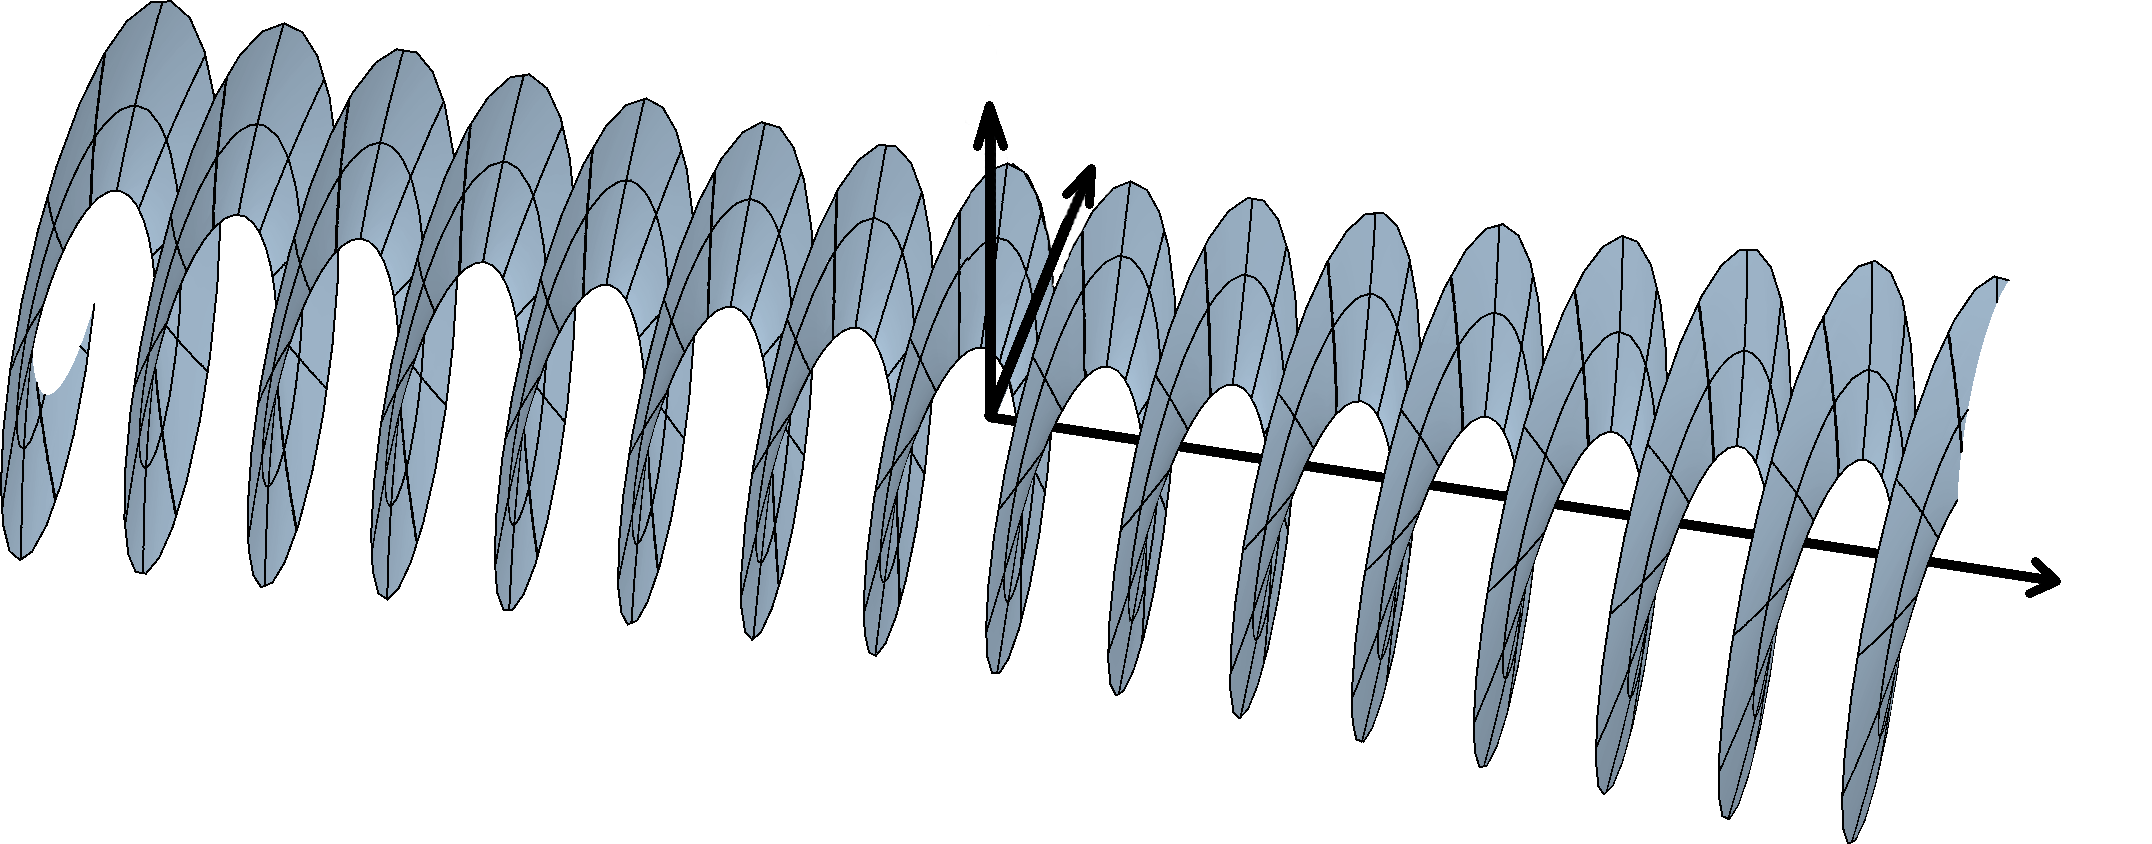
\includegraphics[width=10truecm]{slike/03_Laguerre_faza.png}
\caption{Valovna fronta Laguerre-Gaussovega snopa}
\label{fig:Laguerrova_fronta}
\end{figure}
\end{remark}

\section{Besslov snop}

Poglejmo še poseben primer omejenega snopa, to je \index{Besslov snop}Besslov
snop\footnote{Nemški astronom, matematik in fizik Friedrich Wilhelm Bessel, 1784--1846.}. 
Nastavek za eksaktno rešitev valovne enačbe (enačba~\ref{eq:valovna-skalarna}), 
pri čemer obravnavamo polje skalarno, naj bo
\begin{equation}
E=E_{0}\psi(x,y)e^{i\beta z-i\omega t}.
\end{equation}
Funkcija $\psi$ mora zadoščati Helmholtzevi enačbi\index{Helmholtzeva enačba}
(enačba~\ref{eq:Helmholtz})
\begin{equation}
\nabla_{\perp}^{2}\psi+k_{\perp}^{2}\psi=0
\end{equation}
pri $k_{\perp}^{2}=k^{2}-\beta^{2}$. V cilindričnih
koordinatah ($x=r\cos\varphi$, $y=r\sin\varphi$) se enačba prepiše v 
\begin{equation}
\frac{\partial^2 \psi}{\partial r^2}+ \frac{1}{r}\frac{\partial \psi}{\partial r}
+ \frac{1}{r^2}\frac{\partial^2 \psi}{\partial \varphi^2}+k_{\perp}^{2}\psi=0.
\end{equation}
Rešitve gornje enačbe so s faznim faktorjem pomnožene Besslove funkcije
\begin{equation}
\psi_m(r, \varphi)=J_{m}(k_{\perp}r)e^{im\varphi},
\end{equation}
kjer je $J_{m}$ Besslova funkcija, $m$ pa celo število. Za
$m=0$ je rešitev osnovi Besslov snop
\begin{equation}
E(r,z,t)=E_{0}J_{0}(k_{\perp}r)e^{i\beta z-i \omega t}.
\label{eq:Besslov-snop}
\end{equation}
Valovne fronte Besslovega snopa so ravne 
in snop nima divergence\index{Besslov snop!divergenca}. Vendar pa Besslov snop ni 
omejen v pravem smislu. Za velike oddaljenosti od osi snopa $r$ intenzitetni profil 
namreč pojema kot $I \propto J_{0}^{2}(k_{\perp}r)\sim (2/\pi k_{\perp}r)\cos^{2}(k_{\perp}r-\pi/4)$.
Energija takega snopa ni omejena znotraj efektivnega radija,
kot je to pri Gaussovih snopih. Za konstrukcijo Besslovih snopov
bi (tako kot za konstrukcijo ravnega vala) potrebovali neskončno energije,
kar je seveda nemogoče. Lahko pa ustvarimo dobre približke Besslovih 
snopov, ki imajo pomembne in uporabne lastnosti. 

\begin{figure}[h]
\centering
\def\svgwidth{70truemm} 
\input{slike/03_Bessel_profil.pdf_tex}
\caption{Prečni presek in profil intenzitete Besslovega snopa}
\label{fig:Besslov_presek}
\end{figure}

\begin{remark}
Z uporabo stožčaste leče (aksikona) lahko Gaussov snop
preoblikujemo v približek Besslovega snopa (slika~\ref{fig:Bessel_leca}). 
Na plašču stožčaste leče se namreč Gaussov snop zlomi in valovni vektorji 
nastalega snopa opisujejo stožec, kar je sicer lastnost Besslovih snopov.
Dobljeni snop je približek Besslovega snopa, vendar le na določenem območju, dolgem $z_{max}$.
Znotraj tega območja je divergenca snopa praktično enaka nič. Poleg manjše divergence
imajo ti snopi še lastnost regeneracije. To pomeni, da se snop v senčni strani
za objektom, ki ga osvetljuje (na primer v optični pinceti), regenerira. 
Profil snopa v senčni strani (daleč stran od objekta) je tako enak profilu 
snopa pred objektom. 
\begin{figure}[h]
\centering
\def\svgwidth{90truemm} 
\input{slike/03_Bessel_nastanek.pdf_tex}
\caption{Nastanek približka Besslovega snopa na stožčasti leči}
\label{fig:Bessel_leca}
\end{figure}
\end{remark}

\section{Transformacije snopov z lečami}

Vrnimo se h Gaussovim snopom in poglejmo, kaj se zgodi z njimi pri prehodu
skozi optične elemente\index{Preslikava z lečo}. Začnemo
z enostavno tanko lečo z goriščno razdaljo $f$. V geometrijski optiki
je krivinski radij krogelnega vala, ki izhaja iz točke na osi, kar
enak razdalji do točke. Leča točko na optični osi preslika v točko na osi,
od tod pa sledi, da se krogelni val s krivinskim radijem $R_{1}$
po prehodu skozi lečo spremeni v val s krivinskim radijem $R_{2}$.
Pri tem velja zveza 
\begin{equation}
\frac{1}{R_{1}}-\frac{1}{R_{2}}=\frac{1}{f}.
\label{eq:leca}
\end{equation}
Dogovorimo se, da je krivinski radij v točki $z$ pozitiven, če je središče krožnice pri $z^{\prime}\le z$.

Kako pa je z Gaussovim snopom? Polmer snopa $w$ se pri prehodu 
skozi tanko lečo ne spremeni, zato velja po enačbah (\ref{eq:q-inv}) in 
(\ref{eq:leca}) za kompleksni krivinski radij tik pred lečo in tik za njo
\begin{equation}
\frac{1}{q_{1}}-\frac{1}{q_{2}}=\frac{1}{f}.
\label{eq:preslikava-zveza-leca}
\end{equation}
Kompleksni krivinski radij $q$ je po enačbi~(\ref{eq:q}) linearna 
funkcija koordinate $z$ in za opis Gaussovega snopa zadošča, če
v neki točki $z$ poznamo $q$. Iz realnega dela določimo ukrivljenost front, iz 
imaginarnega pa polmer snopa. Enačba~(\ref{eq:preslikava-zveza-leca}) torej
zadošča za račun prehoda snopa skozi poljuben sistem leč brez aberacij.

Kot primer poglejmo, kako z zbiralno lečo zberemo Gaussov snop.
\begin{figure}[h]
\centering
\def\svgwidth{140truemm} 
\input{slike/03_preslikava.pdf_tex}
\caption{Prehod Gaussovega snopa skozi
tanko lečo. Grlo velikosti $w_{01}$ v oddaljenosti $x_{1}$ od gorišča
leče $F$ se preslika v grlo velikosti $w_{02}$ v oddaljenosti $x_{2}$ od gorišča
leče $F$.}
\label{fig:Prehod-Gaussovega-snopa}
\end{figure}

Vpadni snop naj ima grlo s polmerom $w_{01}$ in parametrom $z_{01}=\pi w_{01}^2/\lambda$. 
Lega grla je 
v točki, ki je za $x_{1}$ oddaljena od levega gorišča leče $F$ (slika
\ref{fig:Prehod-Gaussovega-snopa}). Naj bosta 
\begin{equation}
q_{1}^{F}=x_{1}-iz_{01}\mbox{\hskip1cm in \hskip1cm}q_{2}^{F}=-x_{2}-iz_{02}
\label{eq:qFqF}
\end{equation}
 kompleksna krivinska radija v levem in desnem gorišču, pri čemer je koordinatna os $z$ 
 usmerjena v desno, gledamo pa referenčno glede na lego grla vsakega posameznega snopa. 
 Za vrednosti $q$ tik pred lečo in tik za njo velja tudi
\begin{equation}
q_{1}=q_{1}^{F}+f\mbox{\hskip1cm in \hskip1cm}q_{2}=q_{2}^{F}-f.
\end{equation}
 Od tod z uporabo enačbe~(\ref{eq:preslikava-zveza-leca}) izpeljemo zvezo
za $q$ v goriščih v kompaktni obliki 
\boxeq{eq:qqf}{
q_{1}^{F}q_{2}^{F}=-f^{2}.
}
 Enačba je po obliki podobna enačbi za oddaljenost slike od gorišča v
geometrijski optiki, pomen pa ima drugačen. Uporabimo enačbi~(\ref{eq:qFqF}) in 
zapišimo posebej realni in imaginarni del 
\begin{equation}
x_{1}x_{2}=f^{2}-z_{01}z_{02} \qquad \mathrm{in} \qquad
\frac{x_{1}}{z_{01}}=\frac{x_{2}}{z_{02}}.
\end{equation}
Dobimo enačbi za preslikavo Gaussovega snopa z lečo z goriščno razdaljo $f$.
Prva enačba 
\boxeq{eq:preslikava-grlo}{
x_{2}=\frac{x_{1}f^{2}}{x_{1}^{2}+z_{01}^{2}}
}
določa lego grla preslikanega snopa na desni strani leče, druga pa povečavo
\boxeq{eq:preslikava-povecava}{
\frac{w_{02}}{w_{01}}=\sqrt{\frac{x_{2}}{x_{1}}}.
}
Enačba (\ref{eq:preslikava-grlo}) se ujema z izrazom za preslikavo točke v geometrijski
optiki le, kadar je $z_{01}\ll x_{1}$. Kadar je $z_{01}\gg f$, je
val na leči pri vsakem $x_{1}$ skoraj raven in $x_2 \to 0$, kar pomeni, da leži
grlo na desni strani v gorišču. V praksi za Gaussove snope, ki izhajajo iz laserjev, pogosto ne
velja ne prva ne druga limita, zato je treba uporabiti zapisani izraz 
(enačba~\ref{eq:preslikava-grlo}).
Tudi velikost polmera grla na desni, podana z enačbo (\ref{eq:preslikava-povecava}),
je precej drugačna kot v geometrijski optiki.

Za primer vzemimo snop iz He-Ne laserja\index{Laser!He-Ne} 
(valovna dolžina $632,8~\si{\nano\metre}$), ki ima grlo s 
polmerom $w_{01}=0,5~\si{\milli\metre}$ na izhodnem ogledalu in je $50~\si{\centi\metre}$ 
oddaljeno od leče z goriščno razdaljo $f=25~\si{\centi\metre}$.
Za tak snop je $z_{01}=124~\si{\centi\metre}$. Po enačbi (\ref{eq:preslikava-grlo})
leži grlo za lečo v oddaljenosti $1~\si{\centi\metre}$ od gorišča in torej $26~\si{\centi\metre}$ 
za lečo, po enačbi (\ref{eq:preslikava-povecava})
pa izračunamo polmer $w_{02}=100~\si{\micro\metre}$. Enačbe geometrijske optike bi
dale popolnoma napačen položaj grla $50~\si{\centi\metre}$ za lečo, polmer grla pa 
$0,5~\si{\milli\metre}$. Po drugi strani bi približek, da je vpadni
snop kar raven, dal grlo na desni v gorišču s približno pravim polmerom. Zakaj da približek ravnih 
valov bolj pravilen rezultat, lahko hitro uvidimo, če pogledamo
Rayleighovo dolžino snopa $z_{01}$: 
snop vpada na lečo še v območju bližnjega polja ($x_1 + f < z_{01}$), kjer 
je približno oblike ravnih valov. 

Če postavimo gorišče leče v grlo snopa ($x_{1}=0$), je grlo na
desni strani tudi v gorišču ($x_{2}=0$). Razmerje polmerov grl
na eni in drugi strani leče lahko izračunamo
\begin{equation}
\lim_{x_1 \to 0}~\frac{x_{2}}{x_{1}}=\frac{f^{2}}{z_{01}^{2}} \qquad \textrm{in} \qquad
\frac{w_{02}}{w_{01}}= \frac{f}{z_{01}}.
\end{equation}
Velikost grla na desni strani je tako
\begin{equation}
w_{02}=\frac{\lambda f}{\pi w_{01}}.
\end{equation}
Če želimo doseči kar se da majhno grlo po prehodu skozi lečo, mora biti polmer
vpadnega snopa kar se da velik. Vpadni snop je tako smiselno
razširiti, vendar je polmer snopa lahko največ enak polmeru leče $a$. 
Najmanjša velikost grla, ki jo še lahko dosežemo z zbiralno lečo, je tako 
\boxeq{eq:wmin}{
w_{02~\textrm{min}} = \frac{\lambda f}{\pi a} \sim \lambda.
}
Dobri mikroskopski in fotografski
objektivi dosegajo $f/a\simeq 1$, zato je mogoče z njimi Gaussov snop
zbrati v piko velikosti $\sim\lambda$. 

Omenili smo, da je treba za dosego majhnega polmera grla za lečo snop pred lečo čim bolj razširiti.
Razširitev vpadnega snopa naredimo s teleskopom~(slika~\ref{fig:Prehod-Gaussovega-snopa-teleskop}),
katerega značilnost je, da je razmik med lečama enak vsoti goriščnih razdalj leč in zato gorišči
leč sovpadata. Povečava teleskopa je pri taki postavitvi leč enaka razmerju med goriščnima razdaljama 
(glej nalogo~\ref{teleskop}).

\begin{figure}[h]
\def\svgwidth{145truemm} 
\input{slike/03_teleskop.pdf_tex}
\caption{Prehod Gaussovega snopa
skozi teleskop iz leč z goriščnima razdaljama $f_{1}$ in $f_{2}$. Pri teleskopu
gorišči leč sovpadata.}
\label{fig:Prehod-Gaussovega-snopa-teleskop}
\end{figure}

\begin{definition}
\label{teleskop}
Dve leči z goriščnima razdaljama $f_{1}$ in $f_{2}$ naj bosta na medsebojni
razdalji $d=f_{1}+f_{2}$. Pokaži, da je povečava takega teleskopa enaka  
\begin{equation}
\frac{w_{02}}{w_{01}}=\frac{f_{2}}{f_{1}}.
\label{eq:povecava-teleskop}
\end{equation}
\end{definition}

\section{Matrične (ABCD) preslikave v geometrijski optiki}

Preden se lotimo splošnejšega zapisa preslikav Gaussovega snopa, 
se spomnimo, kako obravnavamo preslikave v geometrijski optiki. 
Slika nastane kot presečišče žarkov,
ki izhajajo iz točke predmeta pred optičnim sistemom. Žarek 
je pravokoten na valovne ploskve, pri čemer moramo vzeti še limito,
ko gre valovna dolžina proti nič. Ukrivljenost valovne fronte je neposredno
povezana s spreminjanjem naklona žarkov, pri čemer bomo privzeli, da so 
nakloni žarkov glede na os majhni.

Žarek v izbrani ravnini $z$ lahko opišemo z dvema parametroma: 
oddaljenostjo $y$ od osi in naklonom $\vartheta$ glede na os sistema. Ti dve količini 
sta med seboj neodvisni in ju sestavimo 
v vektor
\begin{equation}
\left[\begin{array}{c}
y\\
\vartheta
\end{array}\right].
\end{equation}
Preslikavo žarka zapišemo kot matriko, ki deluje na vpadni vektor in ga preslika
v izhodni vektor (slika~\ref{fig:K-matricni-obravnavi})
\begin{equation}
\left[\begin{array}{c}
y_2\\
\vartheta_2
\end{array}\right] = M \left[\begin{array}{c}
y_1\\
\vartheta_1
\end{array}\right].
\end{equation}

\begin{figure}[h]
\centering
\centering
\def\svgwidth{100truemm}
\input{slike/03_k_preslikavam.pdf_tex}
\caption{Preslikave žarkov lahko obravnavamo
z matrikami. Optični element, ki ga predstavlja matrika $M$, 
preslika žarek $(y_{1},\vartheta_{1})$
v $(y_{2},\vartheta_{2})$.}
\label{fig:K-matricni-obravnavi}
\end{figure}

Matrike $M$ so na splošno oblike
\begin{equation}
M = \left[\begin{array}{cc}
A & B\\
C & D
\end{array}\right],
\end{equation}
zato jih imenujemo tudi matrike ABCD\index{Matrike ABCD}. Poglejmo nekaj primerov. 

Pri premiku za $d$ vzdolž osi se zaradi končnega naklona spremeni odmik od osi, naklon pa ostane enak
\begin{equation}
\left[\begin{array}{c}
y_{2}\\
\vartheta_{2}
\end{array}\right]=\left[\begin{array}{c}
y_{1}+d\vartheta_{1}\\
\vartheta_{1}
\end{array}\right].
\end{equation}
To lahko zapišemo v matrični obliki
\begin{equation}
\left[\begin{array}{c}
y_{2}\\
\vartheta_{2}
\end{array}\right]=\left[\begin{array}{cc}
1 & d\\
0 & 1
\end{array}\right]\cdot\left[\begin{array}{c}
y_{1}\\
\vartheta_{1}
\end{array}\right].
\end{equation}
Matrika za premik $d$ vzdolž osi $z$ je tako
\begin{equation}
M= \left[\begin{array}{cc}
1 & d\\
0 & 1
\end{array}\right].
\end{equation}
Poglejmo še matriko za prehod skozi lečo. 
Pri prehodu skozi tanko lečo se spremeni nagib žarka. Če je žarek pred
lečo vzporeden z osjo, gre za lečo skozi gorišče, zato 
\begin{equation}
\left[\begin{array}{c}
y_{2}\\
\vartheta_{2}
\end{array}\right]=\left[\begin{array}{c}
y_{1}\\
-\frac{y_{1}}{f}
\end{array}\right]=\left[\begin{array}{cc}
1 & B\\
-\frac{1}{f} & D
\end{array}\right]\cdot\left[\begin{array}{c}
y_{1}\\
0
\end{array}\right].
\end{equation}
Pri tem koeficientov $B$ in $D$ še ne poznamo. Določimo jih iz drugega pogoja, 
ki pravi, da se žarek, ki gre skozi lečo na osi, ne spremeni
\begin{equation}
\left[\begin{array}{c}
y_{2}\\
\vartheta_{2}
\end{array}\right]=\left[\begin{array}{c}
0\\
\vartheta_{1}
\end{array}\right]=\left[\begin{array}{cc}
1 & B\\
-\frac{1}{f} & D
\end{array}\right]\cdot\left[\begin{array}{c}
0\\
\vartheta_{1}
\end{array}\right].
\end{equation}
 Sledi $B=0$ in $D=1$. Matrika za prehod skozi lečo je tako 
\begin{equation}
M= \left[\begin{array}{cc}
1 & 0\\
-\frac{1}{f} & 1
\end{array}\right].
\end{equation}
Podobno izpeljavo kot za prehod skozi lečo naredimo za odboj na sferičnem zrcalu
s krivinskim radijem $R$. Pripadajoča matrika je 
\begin{equation}
M=\left[\begin{array}{cc}
1 & 0\\
-\frac{2}{R} & 1
\end{array}\right],
\end{equation}
pri čemer je $R>0$ za konkavna zrcala. Matrika za odboj na ravnem zrcalu je identiteta.

Matriko sestavljene optične naprave zapišemo kot produkt matrik posameznih komponent. 
Pri tem moramo paziti na vrstni red množenja, saj množenje matrik ni komutativno.
Matriko preslikave z dvema optičnima elementoma, pri čemer žarek 
najprej preide element z indeksom 1 in nato element z indeksom 2, zapišemo kot 
\begin{eqnarray}
\left[\begin{array}{cc}
A & B\\
C & D
\end{array}\right] & = & \left[\begin{array}{cc}
A_{2} & B_{2}\\
C_{2} & D_{2}
\end{array}\right]\cdot\left[\begin{array}{cc}
A_{1} & B_{1}\\
C_{1} & D_{1}
\end{array}\right]=\left[\begin{array}{cc}
A_{2}A_{1}+B_{2}C_{1} & A_{2}B_{1}+B_{2}D_{1}\\
C_{2}A_{1}+D_{2}C_{1} & C_{2}B_{1}+D_{2}D_{1}
\end{array}\right].
\end{eqnarray}
V sistemu z več elementi zapišemo produkt matrik za vse elemente, 
pri čemer ne smemo pozabiti na premike med elementi.

Poglejmo primer. Žarek naj najprej prepotuje razdaljo $d$, nato pa ga usmerimo
na tanko lečo z goriščno razdaljo $f$. Matrika za celoten prehod je
\begin{eqnarray}
\left[\begin{array}{cc}
A & B\\
C & D
\end{array}\right] & = & \left[\begin{array}{cc}
1 & 0\\
-\frac{1}{f} & 1
\end{array}\right]\cdot\left[\begin{array}{cc}
1 & d\\
0 & 1
\end{array}\right] =  \left[\begin{array}{cc}
1 & d\\
-\frac{1}{f} & -\frac{d}{f}+1
\end{array}\right].
\label{eq:Mdf}
\end{eqnarray}
\begin{remark}
Opisani matrični formalizem je zelo prikladen predvsem za računanje prehoda
svetlobe skozi zapletene optične sisteme, saj ga je prav lahko izvesti z računalnikom. Poleg
tega je enolično povezan z matričnim formalizmom izračuna
kompleksne ukrivljenosti Gaussovih snopov, zato omogoča preprost prenos 
rezultatov geometrijske optike v optiko snopov.
\end{remark}

\section{Linearne racionalne transformacije kompleksnega krivinskega radija}

Poskusimo zdaj zapisati podoben matrični formalizem še za kompleksne krivinske
radije. Za opis Gaussovega snopa zadošča, da v izbrani ravnini $z$ poznamo kompleksni
krivinski radij $q$. Vemo, da je $q$ linearna funkcija
premika po $z$ (enačba~\ref{eq:q}). Izračunali smo tudi že, kako se $q$ 
spremeni pri prehodu skozi tanko lečo (enačba~\ref{eq:preslikava-zveza-leca}). 

Pri premiku iz ravnine $z_1$ v ravnino $z_2$, ki je premaknjena
za $d$, se $q$ spremeni 
\begin{equation}
q_2=q_1+d.
\end{equation}
Po enačbi~(\ref{eq:preslikava-zveza-leca}) je pri prehodu skozi lečo
\begin{equation}
q_2=\frac{q_1f}{f-q_1}=\frac{q_1}{-\frac{q_1}{f}+1}.
\end{equation}
Premik in leča dasta skupaj
\begin{equation}
q_2=\frac{q_1+d}{-\frac{q_1+d}{f}+1}=\frac{q_1+d}{-\frac{q_1}{f}-\frac{d}{f}+1}.
\label{eq:premikleca}
\end{equation}
V vseh treh primerih lahko transformacijo kompleksnega krivinskega radija 
$q$ zapišemo v obliki ulomljene
linearne preslikave 
\boxeq{eq:ulomljena-preslikava}{
q_2=\frac{Aq_1+B}{Cq_1+D}.
}
Ko koeficiente preslikave razvrstimo v matriko 
\begin{equation}
M= \left[\begin{array}{cc}
A & B\\
C & D
\end{array}\right]
\end{equation}
in iz gornjih enačb razberemo koeficiente matrik \index{Matrike ABCD} za opisane 
preslikave, vidimo, da so povsem enaki koeficientom matrik ABCD, ki jih poznamo iz
geometrijske optike. Hitro lahko tudi preverimo, 
da je matrika za premik in lečo, ki jo dobimo iz preslikave (enačba~\ref{eq:premikleca}),
enaka produktu matrike za premik in matrike za lečo
(enačba~\ref{eq:Mdf}). 

Omenimo še eno lastnost matrik ABCD. Kadar po prehodu skozi optične elemente snop svetlobe 
preide v snov z enakim lomnim količnikom kot je bil na začetku, je determinanta matrike 
ABCD enaka 1. V nasprotnem
primeru je determinanta matrike enaka razmerju lomnih količnikov začetne in končne snovi. 
\begin{equation}
\det(M) = AD-BC = \frac{n_1}{n_2}.
\end{equation}
\newpage
\begin{table}[t!]
 \centering
  \begin{tabular}{|c|c|c|} \hline
  Opis prehoda & Skica & Matrika za prehod \\ \hline   
      Prehod skozi prostor za $d$ & \parbox[c]{3cm}{\def\svgwidth{3cm}\input{slike/03_matrika_d.pdf_tex}} & 
      $\begin{bmatrix} 1 & d\\  0 & 1 \end{bmatrix}$ \\ \hline

      Prehod skozi mejo dveh snovi & \parbox[c]{3cm}{\def\svgwidth{3cm}\input{slike/03_matrika_n.pdf_tex}} & 
      $\begin{bmatrix} 1 & 0\\ 0 & \frac{n_{1}}{n_{2}} \end{bmatrix}$ \\ \hline
      
      Prehod skozi konveksno ukrivljeno mejo $R>0$ & \parbox[c]{3cm}{\def\svgwidth{3cm}\input{slike/03_matrika_nR.pdf_tex}} & 
      $\begin{bmatrix} 1 & 0\\ \frac{(n_{1}-n_{2})}{n_{2}R} & \frac{n_{1}}{n_{2}} \end{bmatrix}$ \\ \hline
      
      Prehod skozi konveksno lečo $f>0$ & \parbox[c]{3cm}{\def\svgwidth{3cm}\input{slike/03_matrika_f.pdf_tex}} & 
      $\begin{bmatrix} 1 & 0\\ -\frac{1}{f} & 1 \end{bmatrix}$ \\ \hline
      
      Odboj na konkavnem zrcalu $R>0$ & \parbox[c]{3cm}{\def\svgwidth{3cm}\input{slike/03_matrika_R.pdf_tex}} & 
      $\begin{bmatrix} 1 & 0\\ -\frac{2}{R} & 1 \end{bmatrix}$ \\ \hline    
  \end{tabular}
  \caption{Matrike ABCD za nekaj osnovnih preslikav, ki veljajo tako v 
	  geometrijski optiki kot tudi za izračun preslikave kompleksnega
	  krivinskega radija $q$ Gaussovih snopov.}
\label{fig:Matrike-za-preslikave}
\end{table}

\begin{definition}
Pokaži, da za naslednje prehode veljajo ustrezne matrike ABCD. \\ \\
\begin{tabular}{|c|c|c|} \hline  
      Prehod skozi prostor in lečo & \parbox[c]{3cm}{\def\svgwidth{3cm}\input{slike/03_matrika_df.pdf_tex}} & 
      $\begin{bmatrix} 1 & d\\ -\frac{1}{f} & 1-\frac{d}{f} \end{bmatrix}$ \\ \hline
      \parbox[c]{12em}{Prehod skozi lečo z debelino $d$ 
      in krivinskima radijema $R_1$ in $R_2$}& 
      \parbox[c]{3cm}{\def\svgwidth{3cm}\input{slike/03_matrika_fd.pdf_tex}} & 
      $\begin{bmatrix} 1-\frac{d}{nf_{1}} & \frac{d}{n}\\
      -\frac{1}{f_2}- \frac{1}{f_1}-\frac{d}{nf_1f_2}& 1-\frac{d}{nf_{2}} \end{bmatrix}$
      $f_{i}=\frac{R_{i}}{n-1}$\\ \hline
      Prehod skozi zaporedje plasti & \parbox[c]{3cm}{\def\svgwidth{3cm}\input{slike/03_matrika_nN.pdf_tex}} & 
      $\begin{bmatrix} 1 & \sum_{i=1}^{N}\frac{d_{i}}{n_{i}}\\ 0 & 1 \end{bmatrix}$ \\ \hline 
\end{tabular}
\end{definition}
